\documentclass[10pt]{beamer}

\usetheme[progressbar=frametitle]{metropolis}
\usepackage{appendixnumberbeamer}
\usepackage{booktabs}
\usepackage[scale=2]{ccicons}
\usepackage{color}
\usepackage{pgfplots}
\usepgfplotslibrary{dateplot}
\usetikzlibrary{snakes} 
\usepackage{xspace}
\usetikzlibrary{chains,fit,shapes}
\newcommand{\themename}{\textbf{\textsc{metropolis}}\xspace}

\newcommand{\CalA}{\mathcal{A}}
\newcommand{\CalC}{\mathcal{C}}
\newcommand{\CalP}{\mathcal{P}}
\newcommand{\CalO}{\mathcal{O}}
\newcommand{\CalM}{\mathcal{M}}
\newcommand{\CalN}{\mathcal{N}}
\newcommand{\CalE}{\mathcal{E}}
\newcommand{\CalF}{\mathcal{F}}
\newcommand{\CalH}{\mathcal{H}}
\newcommand{\CalG}{\mathcal{G}}
\newcommand{\CalS}{\mathcal{S}}
\newcommand{\CalT}{\mathcal{T}}
\newcommand{\CalL}{\mathcal{L}}
\newcommand{\CalI}{\mathcal{I}}
\newcommand{\CalJ}{\mathcal{J}}
\newcommand{\CalIC}{{\cal IC}}
\newcommand{\Next}{\textit{next}\xspace}
\newcommand{\Done}{\textit{done}\xspace}
\newcommand{\inputtreshold}{\frac{1}{2}}
\newcommand{\hiddentreshold}{\frac{\omega}{2}}
\newcommand{\outputtreshold}{\frac{\omega}{2}}
\newcommand{\noessay}{e^\bot}
\newcommand{\library}{\ell^\top}
\newcommand{\nolibrary}{\ell^\bot}
\newcommand{\abone}{\Ab_1^\top}
\newcommand{\noabone}{\Ab_1^\bot}
\newcommand{\abtwo}{\Ab_2^\top}
\newcommand{\noabtwo}{\Ab_2^\bot}
\newcommand{\textbook}{t^\top}
\newcommand{\notextbook}{t^\bot}
\newcommand{\essay}{e^\top}
\newcommand{\Def}{\mathit{def}}
\newcommand{\Undef}{\mathit{undef}}
\newcommand{\Atoms}{\mathit{atoms}}
\newcommand{\Comp}{\mathit{c}}
\newcommand{\WComp}{\mathit{wc}}
\newcommand{\ModelsWCS}{\models_{\normalfont\textit{wcs}}}
\newcommand{\udf}{\mbox{\normalfont U}}
\newcommand{\Body}{\mbox{\em Body}}
\newcommand{\Lfp}{\mathsf{lfp}\,}
\newcommand*{\DashedArrow}[1][]{\mathbin{\tikz [baseline=-0.25ex,-latex, dashed,#1] \draw [#1] (0pt,0.5ex) -- (1.3em,0.5ex);}}%


% ------------------------------------------------------------------------------------------------------------------------------------------------------------ %
\newcommand{\coreoverviewex}[1][]{% 1 optional parameter for options for the tikz picture
\def\layersep{3cm}
\begin{tikzpicture}

\draw (0,0) node [rectangle,draw=black,minimum height=5cm, minimum width=3.5cm, text centered, rounded corners = 10pt] (A) {};
\draw (1,-2) node [black, text centered] (C) {$\CalN_{\CalA_\CalP}$};
\only<1>{
\draw (0,0.9) node [gray, text centered] (C) {generate};
\draw (0,0.3) node [gray, text centered] (C) {sequence of};
\draw (0,-0.3) node [gray, text centered] (C) {candidate};
\draw (0,-0.9) node [gray, text centered] (C) {exaplantions};
} \only<2-> {
\draw (0,0.9) node [black, text centered] (C) {$e \leftarrow \top.$};
\draw (0,0.3) node [black, text centered] (C) {$e \leftarrow \bot.$};
\draw (0,-0.3) node [black, text centered] (C) {$t \leftarrow \top.$};
\draw (0,-0.9) node [black, text centered] (C) {$t \leftarrow \bot.$};
}
\draw (7,0) node [rectangle,draw=black,minimum height=5cm, minimum width=3.5cm, text centered,, rounded corners = 10pt] (P) {};
\draw (8,-2) node [black, text centered] (C) {$\CalN_\CalP$};
\only<1>{
\draw (7,0.9) node [gray, text centered] (C) {};
\draw (7,0.3) node [gray, text centered] (C) {is given candidate};
\draw (7,-0.3) node [gray, text centered] (C) {an explanation?};
\draw (7,-0.9) node [gray, text centered] (C) {};
} \only<2-> {
\draw (7,0.9) node [black, text centered] (C) {$\ell \leftarrow e \wedge ab_1.$};
\draw (7,0.3) node [black, text centered] (C) {$\ell \leftarrow t \wedge ab_2.$};
\draw (7,-0.3) node [black, text centered] (C) {$ab_1 \leftarrow \bot.\quad$};
\draw (7,-0.9) node [black, text centered] (C) {$ab_2 \leftarrow \bot.\quad$};
}

\draw (14,0) node [rectangle,draw=black,minimum height=5cm, minimum width=3.5cm, text centered,, rounded corners = 10pt] (S) {};
\draw (15,-2) node [black, text centered] (C) {$\CalN_\CalS$};
\only<1>{
\draw (14,0.3) node [gray, text centered] (C) {sceptical};
\draw (14,-0.3) node [gray, text centered] (C) {consequences};
}
\draw (14,0.9) node [black, text centered] (C) {\only<2-4>{$\emptyset$}};
\draw (14,1.5) node [black, text centered] (C) {\only<5-13>{$\langle \{e, \ell\}, \{ab_1, ab_2\}\rangle$}};
\draw (14,0.9) node [black, text centered] (C) {\only<9-13>{$\cap$}};
\draw (14,0.3) node [black, text centered] (C) {\only<9-13>{$\langle \{t, \ell\}, \{ab_1, ab_2\}\rangle$}};
\draw (14,0.3) node [black, text centered] (C) {\only<14>{$\langle \{\ell\}, \{ab_1, ab_2\}\rangle$}};
\draw (14,-0.3) node [black, text centered] (C) {\only<11-13>{$\cap$}};
\draw (14,-0.9) node [black, text centered] (C) {\only<11-13>{$\dots$}};

\draw (14,-0.9) node [black, text centered] (C) {};

%\draw (15,0) node [rectangle,draw=white,minimum height=3cm, minimum width=2cm, text centered,, rounded corners = 10pt] (O) {}; $t \leftarrow \bot$  $\langle \emptyset, \{t, ab_1, ab_2\}\rangle$

\draw [black,->] (A) -- node [above] {\only<1,2>{candidate}\only<3,4>{$\{e \leftarrow \top\}$}\only<5,6>{$\{e \leftarrow \bot\}$}\only<7,8>{$\{t \leftarrow \top\}$}\only<9,10>{$\dots$}\only<11,12>{$\{e \leftarrow \bot, t \leftarrow \bot\}/\textit{done}$}} (P);
\draw [->, black, rounded corners = 10pt]  (8.75,1) to (9.5,1) to (9.5, 3) to node [above] {\only<1,2,4,6,8,10>{request next candidate}}  (-2.5,3) to (-2.5,1) to (-1.75,1);
\draw [black,->] (P) -- node [above] {\only<1,2>{consequences}\only<4>{$\langle \{e, \ell\}, \{ab_1, ab_2\}\rangle$}\only<6>{$\langle \emptyset, \{e, ab_1, ab_2\}\rangle$}\only<8>{$\langle \{t, \ell\}, \{ab_1, ab_2\}\rangle$}\only<10>{$\dots$}\only<12>{$\langle \emptyset, \{e, t, \ell, ab_1, ab_2\}\rangle$}} (S);

%\draw [black,->] (S) -- node [above] {} (O);

%\draw [->, black, rounded corners = 10pt]  (6,-1) to (7,-1) to (7, -3) to node [below] {whether candidate was positive} (-2,-3) to (-2,-1) to (-1,-1);

\end{tikzpicture}
} 

% ------------------------------------------------------------------------------------------------------------------------------------------------------------ %
\newcommand{\coreoverviewext}[1][]{% 1 optional parameter for options for the tikz picture
\def\layersep{3cm}
\begin{tikzpicture}[trim left=-5.5cm]

\draw (0,0) node [rectangle,draw=black,minimum height=5cm, minimum width=3.5cm, text centered, rounded corners = 10pt] (A) {};
\draw (1,-2) node [black, text centered] (C) {$\CalN_{\CalA_\CalP}$};
\only<1>{
\draw (0,0.9) node [gray, text centered] (C) {generate};
\draw (0,0.3) node [gray, text centered] (C) {sequence of};
\draw (0,-0.3) node [gray, text centered] (C) {candidate};
\draw (0,-0.9) node [gray, text centered] (C) {exaplantions};
} \only<2-> {
\draw (0,0.9) node [black, text centered] (C) {$e \leftarrow \top.$};
\draw (0,0.3) node [black, text centered] (C) {$e \leftarrow \bot.$};
\draw (0,-0.3) node [black, text centered] (C) {$t \leftarrow \top.$};
\draw (0,-0.9) node [black, text centered] (C) {$t \leftarrow \bot.$};
}
\draw (8,0) node [rectangle,draw=black,minimum height=5cm, minimum width=3.5cm, text centered,, rounded corners = 10pt] (P) {};
\draw (9,-2) node [black, text centered] (C) {$\CalN_\CalP$};
\only<1>{
\draw (8,0.9) node [gray, text centered] (C) {};
\draw (8,0.3) node [gray, text centered] (C) {is given candidate};
\draw (8,-0.3) node [gray, text centered] (C) {an explanation?};
\draw (8,-0.9) node [gray, text centered] (C) {};
} \only<2-> {
\draw (8,0.9) node [black, text centered] (C) {$\ell \leftarrow e \wedge ab_1.$};
\draw (8,0.3) node [black, text centered] (C) {$\ell \leftarrow t \wedge ab_2.$};
\draw (8,-0.3) node [black, text centered] (C) {$ab_1 \leftarrow \bot.\quad$};
\draw (8,-0.9) node [black, text centered] (C) {$ab_2 \leftarrow \bot.\quad$};
}

\draw (14,-0.9) node [black, text centered] (C) {};

%\draw (15,0) node [rectangle,draw=white,minimum height=3cm, minimum width=2cm, text centered,, rounded corners = 10pt] (O) {};

\draw [black,->] (A) -- node [above] {\only<1,2>{candidate}\only<3>{$\emptyset$}\only<5>{$\{e\leftarrow\top\}$}\only<9>{$\{e\leftarrow\bot\}$}\only<11>{$\{t\leftarrow\top\}$}\only<15>{$\{t\leftarrow\bot\}$}\only<17>{$\{e\leftarrow\bot, t\leftarrow\bot\}$ / \textit{done}}} (P);
\draw [->, black, rounded corners = 10pt]  (9.75,1) to (10.5,1) to (10.5, 3) to node [above] {\only<1,2,4,6,7,8,10,12,13,14,16>{request next candidate}}  (-2.5,3) to (-2.5,1) to (-1.75,1);
%\draw [black,->] (S) -- node [above] {} (O);

\draw [->, black, rounded corners = 10pt]  (9.75,-1) to (10.5,-1) to (10.5, -3) to node [below] {\only<1,2>{whether candidate was explanation}\only<6,7,8,12,13,14>{positive}\only<4,10,16>{negative}} (-2.5,-3) to (-2.5,-1) to (-1.75,-1);

\end{tikzpicture}
} 

% ------------------------------------------------------------------------------------------------------------------------------------------------------------ %
\newcommand{\coreoverviewcandidates}[1][]{% 1 optional parameter for options for the tikz picture
\def\layersep{3cm}
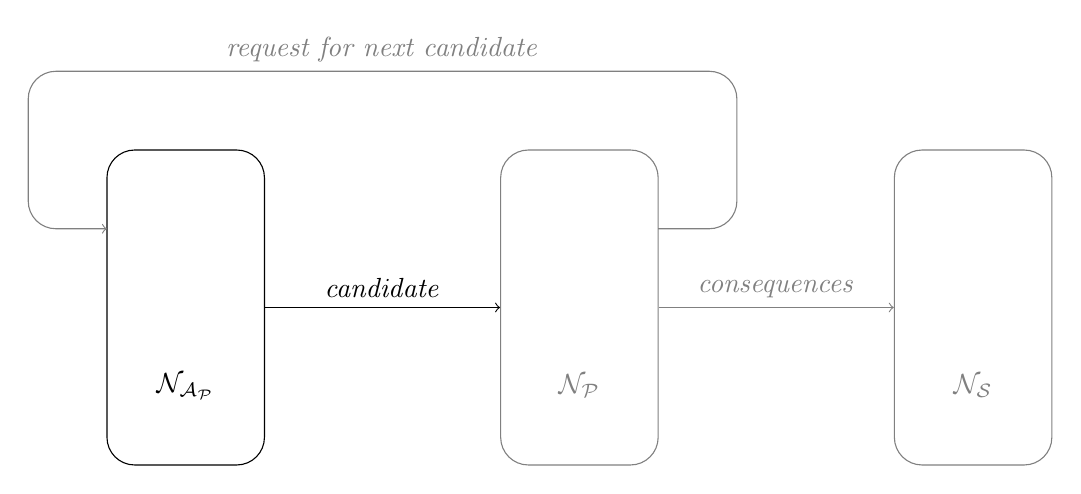
\begin{tikzpicture}

\draw (0,0) node [rectangle,draw=black,minimum height=4cm, minimum width=2cm, text centered, rounded corners = 10pt] (A) {};
\draw (0,-1) node [black, text centered] (C) {$\CalN_{\CalA_{\CalP}}$};
\draw (5,0) node [rectangle,draw=gray,minimum height=4cm, minimum width=2cm, text centered,, rounded corners = 10pt] (P) {};
\draw (5,-1) node [gray, text centered] (C) {$\CalN_\CalP$};
\draw (10,0) node [rectangle,draw=gray,minimum height=4cm, minimum width=2cm, text centered,, rounded corners = 10pt] (S) {};
\draw (10,-1) node [gray, text centered] (C) {$\CalN_\CalS$};

\draw [black,->] (A) -- node [above] {\textit{candidate}} (P);

\draw [->, gray, rounded corners = 10pt]  (6,1) to (7,1) to (7, 3) to node [above] {\textit{request for next candidate}}  (-2,3) to (-2,1) to (-1,1);
\draw [gray,->] (P) -- node [above] {\textit{consequences}} (S);
%\draw [->, black, rounded corners = 10pt]  (6,-1) to (7,-1) to (7, -3) to node [below] {whether candidate was positive} (-2,-3) to (-2,-1) to (-1,-1);

\end{tikzpicture}
} 
% !TEX root = ../thesis.tex
% ------------------------------------------------------------------------------------------------------------------------------------------------------------ %
\newcommand{\elmangeneral}[1][]{% 1 optional parameter for options for the tikz picture
\def\layersep{3cm}
\begin{tikzpicture}

\draw (0,0) node [rectangle,draw=black,minimum height=1cm, minimum width=3cm, text centered] (I) {Input Layer};
\draw (6,0) node [rectangle,draw=black,minimum height=1cm, minimum width=3cm, text centered] (C) {Context Layer};
\draw (3,2.5) node [rectangle,draw=black,minimum height=1cm, minimum width=3cm, text centered] (H) {Hidden Layer};
\draw (3,5) node [rectangle,draw=black,minimum height=1cm, minimum width=3cm, text centered] (O) {Output Layer};

\draw [black,->] (I) -- (H);
\draw [black,->] (C) -- (H);
\draw [black,->] (H) -- (O);
%\draw[gray,->] (H.north) to[out=50,in=-100, looseness=0.8]  (C.south);
\draw [->,dashed, black, rounded corners = 10pt]  (H.north) to (3.05,3.5) to (8,3.5) to (8,-1) to (6,-1) to (6,-0.5);
\end{tikzpicture}
} 
% ------------------------------------------------------------------------------------------------------------------------------------------------------------ %
\newcommand{\elmannc}[1][]{% 1 optional parameter for options for the tikz picture
\def\layersep{3cm}
\begin{tikzpicture}[shorten >=1pt,->,draw=black, node distance=\layersep]
	%\tikzstyle{every pin edge}=[<-,shorten <=1pt]
	%\tikzstyle{neuron}=[circle,fill=black!25,minimum size=17pt,inner sep=0pt]
	\tikzstyle{annot} = [text width=4em, text centered]
	\tikzstyle{neuron}=[circle,draw=black,,minimum size=12pt,inner sep=0pt,text width=2em, text centered]    
    
	% Draw the input layer nodes
	\node[neuron, label=left:$e^\top$] (I-1) at (0,-1) {};
	\node[neuron, label=left:$e^\bot$] (I-2) at (0,-2) {};
	\node[neuron, label=left:$t^\top$] (I-3) at (0,-3) {};
	\node[neuron, label=left:$t^\bot$] (I-4) at (0,-4) {};
	\node[neuron, label=left:$n$] (I-5) at (0,-5) {};
    
	% Draw the context layer nodes
	\foreach \id in {1,...,5}
		\node[neuron] (C-\id) at (0,-6-\id) {};
		
	% Draw the hidden layer nodes
	\foreach \id in {1,...,5}
		\node[neuron] (H-\id) at (\layersep,-3-\id) {};
	
	% Draw the output layer nodes
	\node[neuron, label={[xshift=0.7cm, yshift=-0.2cm]$e^\top$}] (O-1) at (2*\layersep,-4) {};
	\node[neuron, label={[xshift=0.7cm, yshift=-0.2cm]$e^\bot$}] (O-2) at (2*\layersep,-5) {};
	\node[neuron, label={[xshift=0.7cm, yshift=-0.2cm]$t^\top$}] (O-3) at (2*\layersep,-6) {};
	\node[neuron, label={[xshift=0.7cm, yshift=-0.2cm]$t^\bot$}] (O-4) at (2*\layersep,-7) {};
	\node[neuron, label={[xshift=0.7cm, yshift=-0.2cm]$d$}] (O-5) at (2*\layersep,-8) {};

	% Connect every node in the input and context layer with every node in the hidden layer.
	\foreach \source in {1,...,5}
		 \foreach \dest in {1,...,5} {
           		\path (I-\source.east) edge (H-\dest.west);
			\path (C-\source.east) edge (H-\dest.west);
			\path (H-\source.east) edge (O-\dest.west);
		}
            
	% Connect each node in the output layer with the context layer
	\draw [->,dashed, black, rounded corners = 5pt] (3.4,-8) to (4,-8) to (4,-11.5) to (-0.8,-11.5) to (-0.8,-11) to (-0.4,-11);
	\draw [->,dashed, black, rounded corners = 10pt] (3.4,-7) to (4.2,-7) to (4.2,-11.7) to (-1.0,-11.7) to (-1.0,-10) to (-0.4,-10);
	\draw [->,dashed, black, rounded corners = 10pt] (3.4,-6) to (4.4,-6) to (4.4,-11.9) to (-1.2,-11.9) to (-1.2,-9) to (-0.4,-9);
	\draw [->,dashed, black, rounded corners = 10pt] (3.4,-5) to (4.6,-5) to (4.6,-12.1) to (-1.4,-12.1) to (-1.4,-8) to (-0.4,-8);
	\draw [->,dashed, black, rounded corners = 10pt] (3.4,-4) to (4.8,-4) to (4.8,-12.3) to (-1.6,-12.3) to (-1.6,-7) to (-0.4,-7);
	
	% Annotate the layers
	\node[annot,above of=I-1, node distance=1cm] {Input layer};
	\node[annot,above of=C-1, node distance=1cm] {Context layer};
	\node[annot,above of=H-1, node distance=1cm] (hl) {Hidden layer};
	\node[annot,above of=O-1, node distance=1cm] {Output layer};
\end{tikzpicture}
} 
% ------------------------------------------------------------------------------------------------------------------------------------------------------------ %
\newcommand{\elmanmin}[1][]{% 1 optional parameter for options for the tikz picture
\def\layersep{3cm}
\begin{tikzpicture}[shorten >=1pt,->,draw=black, node distance=\layersep]
	%\tikzstyle{every pin edge}=[<-,shorten <=1pt]
	%\tikzstyle{neuron}=[circle,fill=black!25,minimum size=17pt,inner sep=0pt]
	\tikzstyle{annot} = [text width=4em, text centered]
	\tikzstyle{neuron}=[circle,draw=black,,minimum size=12pt,inner sep=0pt,text width=2em, text centered]    
    
	% Draw the input layer nodes
	\node[neuron, label=left:$e^\top$] (I-1) at (0,-1) {};
	\node[neuron, label=left:$e^\bot$] (I-2) at (0,-2) {};
	\node[neuron, label=left:$t^\top$] (I-3) at (0,-3) {};
	\node[neuron, label=left:$t^\bot$] (I-4) at (0,-4) {};
	\node[neuron, label=left:$n$] (I-5) at (0,-5) {};
	\node[neuron, black, label=left:$e$] (I-6) at (0,-6) {};
    
	% Draw the context layer nodes
	\foreach \id in {1,...,5}
		\node[neuron] (C-\id) at (0,-7-\id) {};
		
	% Draw the hidden layer nodes
	\foreach \id in {1,...,5}
		\node[neuron] (H-\id) at (\layersep,-3-\id) {};
	
	% Draw the output layer nodes
	\node[neuron, label={[xshift=0.7cm, yshift=-0.2cm]$e^\top$}] (O-1) at (2*\layersep,-4) {};
	\node[neuron, label={[xshift=0.7cm, yshift=-0.2cm]$e^\bot$}] (O-2) at (2*\layersep,-5) {};
	\node[neuron, label={[xshift=0.7cm, yshift=-0.2cm]$t^\top$}] (O-3) at (2*\layersep,-6) {};
	\node[neuron, label={[xshift=0.7cm, yshift=-0.2cm]$t^\bot$}] (O-4) at (2*\layersep,-7) {};
	\node[neuron, label={[xshift=0.7cm, yshift=-0.2cm]$d$}] (O-5) at (2*\layersep,-8) {};

	% Connect every node in the input and context layer with every node in the hidden layer.
	\foreach \source in {1,...,5}{
		 \foreach \dest in {1,...,5} {
           		\path (I-\source.east) edge (H-\dest.west);
			\path (C-\source.east) edge (H-\dest.west);
			\path (H-\source.east) edge (O-\dest.west);
		}
	}
	\foreach \dest in {1,...,5} 
           	\path [black] (I-6.east) edge (H-\dest.west);
            
	% Connect each node in the output layer with the context layer
	\draw [->,dashed, black, rounded corners = 5pt] (3.4,-8) to (4,-8) to (4,-12.5) to (-0.8,-12.5) to (-0.8,-12) to (-0.4,-12);
	\draw [->,dashed, black, rounded corners = 10pt] (3.4,-7) to (4.2,-7) to (4.2,-12.7) to (-1.0,-12.7) to (-1.0,-11) to (-0.4,-11);
	\draw [->,dashed, black, rounded corners = 10pt] (3.4,-6) to (4.4,-6) to (4.4,-12.9) to (-1.2,-12.9) to (-1.2,-10) to (-0.4,-10);
	\draw [->,dashed, black, rounded corners = 10pt] (3.4,-5) to (4.6,-5) to (4.6,-13.1) to (-1.4,-13.1) to (-1.4,-9) to (-0.4,-9);
	\draw [->,dashed, black, rounded corners = 10pt] (3.4,-4) to (4.8,-4) to (4.8,-13.3) to (-1.6,-13.3) to (-1.6,-8) to (-0.4,-8);
	
	% Annotate the layers
	\node[annot,above of=I-1, node distance=1cm] {Input layer};
	\node[annot,above of=C-1, node distance=1cm] {Context layer};
	\node[annot,above of=H-1, node distance=1cm] (hl) {Hidden layer};
	\node[annot,above of=O-1, node distance=1cm] {Output layer};
\end{tikzpicture}
} 
\input{figures/jordan}

% ------------------------------------------------------------------------------------------------------------------------------------------------------------ %
\newcommand{\tape}[1][]{% 1 optional parameter for options for the tikz picture
\begin{tikzpicture}
\tikzstyle{every path}=[very thick]

\edef\sizetape{0.7cm}
\tikzstyle{tmtape}=[draw,minimum size=\sizetape]
\tikzstyle{tmhead}=[arrow box,draw,minimum size=.8cm,arrow box
arrows={east:.25cm, west:0.4cm}]

%% Draw TM tape
\begin{scope}[start chain=1 going right,node distance=-0.15mm]
    \node [on chain=1,tmtape] {\only<3,4>{\color{brown}}{$\emptyset$}};
    \node [on chain=1,tmtape] {\only<5-8>{\color{brown}}$\{e \leftarrow \top\}$};
    \node [on chain=1,tmtape] {\only<9,10>{\color{brown}}$\{e \leftarrow \bot\}$};
    \node [on chain=1,tmtape] {\only<11-14>{\color{brown}}$\{t \leftarrow \top\}$};
    \node [on chain=1,tmtape] {\only<15,16>{\color{brown}}{$\{t \leftarrow\bot\}$}};
    \node [on chain=1,tmtape] {\only<8-17>{\color{gray}}$\{\only<7>{\color{brown}}{e \leftarrow \top}\only<7>{\color{black}}, t\leftarrow \top\}$};
    \node [on chain=1,tmtape] {\only<8-17>{\color{gray}}$\{\only<7>{\color{brown}}{e\leftarrow \top}\only<7>{\color{black}}, t \leftarrow \bot\}$};
    \node [on chain=1,tmtape] {\only<14-17>{\color{gray}}$\{e\leftarrow\bot, \only<13>{\color{brown}}{t\leftarrow\top}\only<13>{\color{black}}{\}}$};
    \node [on chain=1,tmtape] {\only<17>{\color{brown}}{$\{e\leftarrow \bot, t\leftarrow\bot\}$}};
\end{scope}
\end{tikzpicture}}
% !TEX root = ../thesis.tex

\newcommand{\candidatestree}[1][]{% 1 optional parameter for options for the tikz picture
\begin{tikzpicture}[grow=right, ->,
  baseline,
  level distance=20mm,
  text depth=.1em,
  text height=.8em,
  level distance=80pt,
  level 1/.style={sibling distance=40em},
  level 2/.style={sibling distance=45em},
  level 3/.style={sibling distance=20em},
  level 4/.style={sibling distance=10em},
  level 5/.style={sibling distance=5em}]
\node {0000}
    child { node {done} edge from parent[solid] }
    child {
        node {1000}  edge from parent[dashed]     
        child {
		node {0100} edge from parent[solid]
		child { 
			node {0010} edge from parent[solid]
			child { 
				node {0001} edge from parent[snake]
				child { 
					node {done} edge from parent[snake] 
				}
			}
		}
		child {
			node {0010}
			edge from parent[dashed]
			child { 
				node {0001} edge from parent[solid]
				child { 
					node {done} edge from parent[solid] 
				}
				child { 
					node {0101} edge from parent[dashed]
					child { 
						node {done} edge from parent[solid,snake] 
					}
				}
			}
			child {
				node {0001} edge from parent[dashed]
				child {
					node {0110} edge from parent[solid]
					child { 
						node {done} edge from parent[solid,snake] 
					}
				}
				child { 
					node {0110} edge from parent[dashed]
					child { 
						node {0101} edge from parent[solid,snake]
						child { 
							node {done} edge from parent[solid,snake] 
						}
					}
				}
			}
		}
	}
	child {
                node {0100} edge from parent[dashed]
                	child {
			node {0010} edge from parent[solid]
			child {
				node {0001} edge from parent[solid]
				child { node {done} edge from parent[solid] }
				child { 
					node {1001} edge from parent[dashed]
					child { 
						node {done} edge from parent[solid,snake] 
					}
				}
			}
			child {
				node {0001} edge from parent[dashed]
				child {
					node {1010}
					edge from parent[solid]
					child { 
						node {done} edge from parent[solid,snake] 
					}
				}
				child {
					node {1010}
					edge from parent[dashed]
					child {
						node {1001} edge from parent[solid,snake]
						child { 
							node {done} edge from parent[solid,snake] 
						}
					}
				}
			}
		}
		child {
			node {0010} edge from parent[dashed]
			child {
				node {0001}
				edge from parent[solid]
				child {
					node {done}
					edge from parent[solid]
				}
				child {
					node {1001} edge from parent[dashed]
					child {
						node {0101} edge from parent[solid, snake]
						child {
							node {done} edge from parent[solid, snake]
						}
					}
				}
			}
			child {
				node {0001} edge from parent[dashed]
				child {
					node {1010} edge from parent[solid]
					child {
						node {0110} edge from parent[solid, snake]
						child { 
							node {done} edge from parent[solid,snake]
						}
					}
				}
				child {
					node {1010} edge from parent[dashed]
					child { 
						node {1001} edge from parent[solid, snake] 
						child {
							node {0110} edge from parent[solid,snake] 
							child { 
								node {0101} edge from parent[solid,snake] 
								child { 
									node {done} edge from parent[solid,snake]
								}
							}
						}
					}
				}
			}
		}
	}
    };
\end{tikzpicture}
}
\title{Bounded Skeptical Reasoning}
%\subtitle{Human Reasoning}
\date{\today}
\date{}
\author{Isabelly Lour\^{e}do Rocha}
%\institute{Technische Universit\"{a}t Dresden}
%\titlegraphic{\hfill\includegraphics[height=1.5cm]{figures/logo.jpg}}

\begin{document}

\maketitle

\begin{frame}{Table of contents}
  \setbeamertemplate{section in toc}[sections numbered]
  \tableofcontents[hideallsubsections]
\end{frame}

\section{Introduction}
%----------------------------------------------------------------------------------------------------------%
\begin{frame}[fragile]{Abductive Sceptical Reasoning}

\uncover<1->{\textbf{Byrne's suppression task}} \\\vspace*{-1mm}
\color{gray}{\tiny Ruth MJ Byrne. Suppressing valid inferences with conditionals. In: Cognition. (1989)}

\uncover<2->{\textit{\color{black}{If she has an essay to write, then she will study late in the library.\\}}}
\uncover<3->{\textit{\color{black}{If she has a textbook to read, then she will study late in the library.}}}

\begin{itemize}
\uncover<4->{\item \textbf{Observation}: She will study late in the library}
\uncover<5->{\item Does it follow that \textit{she has an essay to write}?}
\uncover<6->{\item \textbf{Explanations}: 
	\begin{itemize}
		\uncover<7->{\item She has an essay to write}
		\uncover<8->{\item She has a textbook to read}
	\end{itemize}
}
\end{itemize}

\uncover<9->{\color{black}{\textbf{Wason's selection task}}\\\vspace*{-1mm}
\color{gray}{\tiny Peter C Wason. Reasoning about a rule. In: The Quarterly journal of experimental psychology. (1968)}}\\
\uncover<10->{\color{black}{\textbf{Syllogistic reasoning}}\\\vspace*{-1mm}
\color{gray}{\tiny Ana Oliveira da Costa, Emmanuelle-Anna Dietz Saldanha, Steffen H\"{o}lldobler, and Marco Ragni. }\\\vspace*{-2mm}
{\tiny A computational logic approach to human syllogistic reasoning. In: Conference of the Cognitive Science Society (2017)}}

\end{frame}
%----------------------------------------------------------------------------------------------------------%
\section{Sceptical Reasoning Framework}
%----------------------------------------------------------------------------------------------------------%
\begin{frame}{Computing Abductive Sceptical Consequences}

\begin{block}
{\tiny \color{gray}{Emmanuelle-Anna Dietz Saldanha, Steffen H\"{o}lldobler, Carroline Dewi Puspa Kencana Ramli, and Luis Palacios Medinacelli. \\
A Core Method for the Weak Completion Semantics with Skeptical Abduction. In: JAIR (accepted). (2017)}}
\end{block}

\begin{itemize}
	\uncover<2->{\item \textbf{Observation}: She will study late in the library ($\ell$)}
\end{itemize}

\begin{figure}
\scalebox{0.6}{\coreoverviewex}
\label{fig:coreoverview}
\end{figure}

\end{frame}
%----------------------------------------------------------------------------------------------------------%
\begin{frame}{Candidate Explanations' Exponential Growth}

  \begin{figure}
    \begin{tikzpicture}
      \begin{axis}[
        mlineplot,
        xlabel={\# Undefined Atoms},
        ylabel={\# Candidate Explanations},
        width=0.9\textwidth,
        height=6cm,
        xtick={1,...,5},
      ]
      \addplot plot coordinates {(1, 3) (2, 9) (3, 27) (4, 81) (5, 243)};
      \end{axis}
    \end{tikzpicture}
  \end{figure}

\end{frame}
%----------------------------------------------------------------------------------------------------------%
\section{Generating Candidate Explanations}
%----------------------------------------------------------------------------------------------------------%
\begin{frame}{Current Approach}
\begin{itemize}
\uncover<1->{\item \color{black}{McCulloch Pitts network} \\\vspace*{-1mm}
\color{gray}{\tiny Warren S McCulloch and Walter Pitts. A logical calculus of the ideas immanent in nervous activity.}\\\vspace*{-2mm}
{\tiny In: The bulletin of mathematical biophysics. (1943)}}
\uncover<2->{\item \color{black} Generates static pre-defined sequence}
\uncover<3->{\item Restricts candidate explanations to \textit{non-complementary}}
	\begin{itemize}
		\uncover<4->{\item Complementary candidate}

			\uncover<5->{ $e \leftarrow \top, e \leftarrow \bot$}\\
			\uncover<6->{ $e \leftarrow \top \vee \bot$}\\
			\uncover<7->{ $e \leftarrow \top$}\\

	\end{itemize}
\end{itemize}
\end{frame}
%----------------------------------------------------------------------------------------------------------%
\begin{frame}{Minimal Candidate Explanations}
\begin{itemize}
\uncover<1->{\item \textbf{Motivation}: Explanations are monotonic}
\uncover<2->{\item \textbf{Definition}: Candidate explanation $\CalC$ is \textit{minimal} if it does not exist $\CalC' \subset \CalC$, such that
	\begin{itemize}
		\item $\CalC' \cup \CalP \ModelsWCS \CalO$
	\end{itemize}
}\uncover<3->{
\item \textbf{Consequence}: Cardinality constraint to the sequence of candidates }
\uncover<4->{
\item \textbf{How to do}}
	\begin{itemize}
		\uncover<5->{\item Feed back the information whether a candidate was an explanation}
		\uncover<6->{\item Store and use this information to block the generation of candidates which are supersets of known explanations}
	\end{itemize}
\end{itemize}
\end{frame}
%----------------------------------------------------------------------------------------------------------%
\begin{frame}{Minimal Candidate Explanations}

\uncover<2->{
\textbf{Observation}: She will study late in the library ($\ell$)

\vspace*{0.1cm}
\begin{figure}
\scalebox{0.6}{\tape}
\end{figure}
}
\begin{figure}
\begin{centering}
\scalebox{0.6}{\coreoverviewext}
\end{centering}
\end{figure}

\end{frame}
%----------------------------------------------------------------------------------------------------------%
\begin{frame}{Minimal Candidate Explanations}
\uncover<1->{Cognitive adequacy\\\vspace*{1mm}
\color{gray}{\tiny Gerhard Strube. The role of cognitive science in knowledge engineering.\\\vspace*{-2mm}
In: Contemporary knowledge engineering and cognition. Springer, 1992.}}

\begin{itemize}
\uncover<2->{\item Many different possible orderings}
\begin{itemize}
\uncover<3->{\item No minimality \\
$n!$, $n$ is the number of candidate explanations }\\
\uncover<4->{\textbf{2 undefined atoms}: $9! = 362.880$
}\uncover<5->{
\item With minimality \\
$\displaystyle \prod_{i = 0}^{k} c_i!$, $c_i$ is the number of candidates with cardinality $i$ \\}
\uncover<6->{\textbf{2 undefined atoms}: $1! * 4 !* 4! = 576$
}
\end{itemize}
\end{itemize}
\end{frame}
%----------------------------------------------------------------------------------------------------------%
\section{Recurrent Networks}
%----------------------------------------------------------------------------------------------------------%
\begin{frame}{Recurrent Network}
\begin{itemize}
\uncover<1->{\item Designed to learn sequential or time-varying sequences
} \uncover<2->{\item Internal memory to maintain previous state
} \uncover<3->{\item Several applications
\begin{itemize}
	} \uncover<4->{\item Pattern recognition
	} \uncover<5->{\item Language processing
\end{itemize}
} \uncover<6->{\item Two fundamental types
\begin{itemize}
} \uncover<7->{\item Jordan networks \\\vspace*{-1mm}
\color{gray}{\tiny Michael I Jordan. Serial order: A parallel distributed processing approach. (1997)}
} \uncover<8->{\item\color{black}{Elman networks}\\\vspace*{-1mm}
\color{gray}{\tiny Jeffrey L Elman. Representation and structure in connectionist models. (1989)}
}
\end{itemize}
\end{itemize}
\end{frame}
%----------------------------------------------------------------------------------------------------------%
\begin{frame}{Jordan Networks}
\begin{figure}
\scalebox{0.6}{\jordangeneral}
\label{fig:coreoverview}
\end{figure}
\end{frame}
%----------------------------------------------------------------------------------------------------------%
\begin{frame}{Elman Networks}
\begin{figure}
\scalebox{0.6}{\elmangeneral}
\label{fig:coreoverview}
\end{figure}
\end{frame}
%----------------------------------------------------------------------------------------------------------%
\begin{frame}{Generating Arbitrary Sequences}
\begin{figure}
\scalebox{0.5}{\elmanmin}
\label{fig:coreoverview}
\end{figure}
\end{frame}
%----------------------------------------------------------------------------------------------------------%
\begin{frame}{Generating Arbitrary Sequences}
\begin{itemize}
\uncover<1->{\item Training and testing data
	\begin{itemize}
	} \uncover<2->{\item Random activation of unit \textit{next} ($n$)
	} \uncover<3->{\item Random activation of unit \textit{explanation} ($e$)
	\end{itemize}
} \uncover<4->{\item Supervised learning
} \uncover<5->{\[
\mbox{expected output } = 
\begin{cases}
	\text{next candidate}, 	& \text{if unit \textit{next} is active }\\
	\text{current candidate},	& \text{otherwise}
\end{cases}
\]
} \uncover<6->{\item \textbf{Training}: Back-propagation 
} \uncover<7->{\item \textbf{Testing}: Mean absolute error
} \uncover<8->{\item 10-fold cross validation}
\end{itemize}
\end{frame}
%----------------------------------------------------------------------------------------------------------%
\begin{frame}{Generating Arbitrary Sequences}
\begin{itemize}
\uncover<1->{\item What is the ideal number of hidden units?}
	\begin{itemize}
	\uncover<2->{\item \textbf{Too few}: underfitting }
	\uncover<3->{\item \textbf{Too many}: overfitting}
	\end{itemize}
\end{itemize}
\uncover<4->{    \begin{figure}
    \scalebox{0.6}{
    \begin{tikzpicture}
      \begin{axis}[
        mlineplot,
        xlabel={\# Hidden Units},
        ylabel={Mean Absolute Error},
        width=0.9\textwidth,
        height=6cm,
        xtick={1,...,10},
      ]
      \addplot plot coordinates {(1, 0.2893350) (2, 0.2893350) (3, 0.2893350) (4, 0.3183645) (5, 0.2893350) (6, 0.2893350) (7, 0.2804612) (8, 0.2117288) (9, 0.0000000) (10, 0.0000000)};      
       \addplot plot coordinates {(1, 0.2893350) (2, 0.2893350) (3, 0.2893350) (4, 0.2893350) (5, 0.2893350) (6, 0.2780525) (7, 0.2448220) (8, 0.2280523) (9, 0.0000000) (10, 0.0000000)};
       \legend{Elman, Jordan}
      \end{axis}
    \end{tikzpicture}
    
    }
    \end{figure}}
\end{frame}
%----------------------------------------------------------------------------------------------------------%
\begin{frame}{Generating Arbitrary Sequences}
    \begin{figure}
    \begin{tikzpicture}
      \begin{axis}[
        legend style={at={(1,0)},anchor=south east},
        mlineplot,
        xlabel={\# Abducibles},
        ylabel={Optimal \# Hidden Units},
        width=0.9\textwidth,
        height=6cm,
        xtick={2,4,6},
      ]
       \legend  {Elman, Jordan}
      \addplot plot coordinates {(2, 4) (4, 9) (6, 13)};      
       \addplot plot coordinates {(2, 4) (4, 9) (6, 14)};
       
      \end{axis}
    \end{tikzpicture}
  \end{figure}
\end{frame}
%----------------------------------------------------------------------------------------------------------%
\begin{frame}{Generating Arbitrary Sequences}
\begin{itemize}
\uncover<1->{\item Advantages of new approach}
\begin{itemize}
	\uncover<2->{\item Results can be generalised}
		\begin{itemize}
		\uncover<3->{\item Any set of abducibles}
		\uncover<4->{\item Different sequence orderings}
		\end{itemize}
	\uncover<5->{\item Learning}
	\uncover<6->{\item Anytime behaviour}
\uncover<7->{\item Automatisation}
	\begin{itemize}
		\uncover<8->{\item Generation of data}
		\uncover<9->{\item Training and testing via k-fold cross-validation}
		\uncover<10->{\item Plot of the experiment outcome}
	\end{itemize}
\uncover<11->{\item Facility to test variations of the problem}
\end{itemize}
\end{itemize}
\end{frame}
%----------------------------------------------------------------------------------------------------------%
\section{Psychological Experiments}
%----------------------------------------------------------------------------------------------------------%
\begin{frame}{Psychological Experiments}
\begin{itemize}
\uncover<1->{\item \textbf{Hypothesis:} Only minimal candidate explanations are considered}
\begin{itemize}
\uncover<2->{\item \textbf{Observation}: She will study late in the library}
\uncover<3->{\item \textbf{Explanations}: 
	\begin{itemize}
		\uncover<4->{\item \only<12>\textbf{She has an essay to write}}
		\uncover<5->{\item \only<12>\textbf{She has a textbook to read}}
		\uncover<6->{\item \only<9>\textbf{She has an essay to write and a textbook to read}}
	\end{itemize}
}
\uncover<7->{\item Does it follow that \textit{she has an essay to write}?}
	\begin{itemize}
		\uncover<8->{\item No minimality}\uncover<10->{: $\approx$100\% yes}
		\uncover<11->{\item Minimality}\uncover<13->{: $\approx$50\% yes}
	\end{itemize}
\end{itemize}
\end{itemize}
\end{frame}
%----------------------------------------------------------------------------------------------------------%
\begin{frame}{Open Questions}
\begin{itemize}
\uncover<1->{\item Do humans consider only basic explanations?}
\uncover<2->{\item Are the candidate explanations sequentially generated?}
\uncover<3->{\item Are complementary candidates not considered? }
\uncover<4->{\item Do humans generate all the candidates?}
\uncover<5->{\item If a bound is applied, how is this bound characterised? }
\end{itemize}
\end{frame}
%----------------------------------------------------------------------------------------------------------%
\section{Contributions}
%----------------------------------------------------------------------------------------------------------%
\begin{frame}{Contributions}
\begin{itemize}
\uncover<2->{ \item Optimisation of sceptical abduction
	\begin{itemize}
	} \uncover<3->{ \item Reducing number of candidate explanations generated
	} \uncover<4->{ \item Minimality constraint
	\end{itemize}
} \uncover<5->{ \item Elman or Jordan network }
	\begin{itemize}
	\uncover<6->{ \item Learning arbitrary sequences of candidate explanations}
	\end{itemize}
\uncover<7->{ \item Bounded reasoning}
	\begin{itemize}
	\uncover<8->{ \item Anytime behaviour}
	\end{itemize}
\end{itemize}
\end{frame}
%----------------------------------------------------------------------------------------------------------%
{
\begin{frame}[standout]
  Thank you!
\end{frame}
}
\end{document}

